\documentclass{beamer}
\usepackage{amsmath,graphics}
\usepackage{amssymb}

\usetheme{default}
\usepackage{xcolor}

\definecolor{solarizedBase03}{HTML}{002B36}
\definecolor{solarizedBase02}{HTML}{073642}
\definecolor{solarizedBase01}{HTML}{586e75}
\definecolor{solarizedBase00}{HTML}{657b83}
\definecolor{solarizedBase0}{HTML}{839496}
\definecolor{solarizedBase1}{HTML}{93a1a1}
\definecolor{solarizedBase2}{HTML}{EEE8D5}
\definecolor{solarizedBase3}{HTML}{FDF6E3}
\definecolor{solarizedYellow}{HTML}{B58900}
\definecolor{solarizedOrange}{HTML}{CB4B16}
\definecolor{solarizedRed}{HTML}{DC322F}
\definecolor{solarizedMagenta}{HTML}{D33682}
\definecolor{solarizedViolet}{HTML}{6C71C4}
%\definecolor{solarizedBlue}{HTML}{268BD2}
\definecolor{solarizedBlue}{HTML}{134676}
\definecolor{solarizedCyan}{HTML}{2AA198}
\definecolor{solarizedGreen}{HTML}{859900}
\definecolor{myBlue}{HTML}{162DB0}%{261CA4}
\setbeamercolor*{item}{fg=myBlue}
\setbeamercolor{normal text}{fg=solarizedBase03, bg=solarizedBase3}
\setbeamercolor{alerted text}{fg=myBlue}
\setbeamercolor{example text}{fg=myBlue, bg=solarizedBase3}
\setbeamercolor*{frametitle}{fg=solarizedRed}
\setbeamercolor*{title}{fg=solarizedRed}
\setbeamercolor{block title}{fg=myBlue, bg=solarizedBase3}
\setbeameroption{hide notes}
\setbeamertemplate{note page}[plain]
\beamertemplatenavigationsymbolsempty
\usefonttheme{professionalfonts}
\usefonttheme{serif}

\usepackage{fourier}

\def\vec#1{\mathchoice{\mbox{\boldmath$\displaystyle#1$}}
{\mbox{\boldmath$\textstyle#1$}}
{\mbox{\boldmath$\scriptstyle#1$}}
{\mbox{\boldmath$\scriptscriptstyle#1$}}}
\definecolor{OwnGrey}{rgb}{0.560,0.000,0.000} % #999999
\definecolor{OwnBlue}{rgb}{0.121,0.398,0.711} % #1f64b0
\definecolor{red4}{rgb}{0.5,0,0}
\definecolor{blue4}{rgb}{0,0,0.5}
\definecolor{Blue}{rgb}{0,0,0.66}
\definecolor{LightBlue}{rgb}{0.9,0.9,1}
\definecolor{Green}{rgb}{0,0.5,0}
\definecolor{LightGreen}{rgb}{0.9,1,0.9}
\definecolor{Red}{rgb}{0.9,0,0}
\definecolor{LightRed}{rgb}{1,0.9,0.9}
\definecolor{White}{gray}{1}
\definecolor{Black}{gray}{0}
\definecolor{LightGray}{gray}{0.8}
\definecolor{Orange}{rgb}{0.1,0.2,1}
\setbeamerfont{sidebar right}{size=\scriptsize}
\setbeamercolor{sidebar right}{fg=Black}

\renewcommand{\emph}[1]{{\textcolor{solarizedRed}{\itshape #1}}}

\newcommand\tay{T}
\newcommand\dd{\mathrm d}
\newcommand\eul{\mathrm e}

\newcommand\cA{\mathcal A}
\newcommand\cB{\mathcal B}
\newcommand\cC{\mathcal C}
\newcommand\cD{\mathcal D}
\newcommand\cE{\mathcal E}
\newcommand\cF{\mathcal F}
\newcommand\cG{\mathcal G}
\newcommand\cH{\mathcal H}
\newcommand\cI{\mathcal I}
\newcommand\cJ{\mathcal J}
\newcommand\cK{\mathcal K}
\newcommand\cL{\mathcal L}
\newcommand\cM{\mathcal M}
\newcommand\cN{\mathcal N}
\newcommand\cO{\mathcal O}
\newcommand\cP{\mathcal P}
\newcommand\cQ{\mathcal Q}
\newcommand\cR{\mathcal R}
\newcommand\cS{\mathcal S}
\newcommand\cT{\mathcal T}
\newcommand\cU{\mathcal U}
\newcommand\cV{\mathcal V}
\newcommand\cW{\mathcal W}
\newcommand\cX{\mathcal X}
\newcommand\cY{\mathcal Y}
\newcommand\cZ{\mathcal Z}

\newcommand\fA{\mathfrak A}
\newcommand\fB{\mathfrak B}
\newcommand\fC{\mathfrak C}
\newcommand\fD{\mathfrak D}
\newcommand\fE{\mathfrak E}
\newcommand\fF{\mathfrak F}
\newcommand\fG{\mathfrak G}
\newcommand\fH{\mathfrak H}
\newcommand\fI{\mathfrak I}
\newcommand\fJ{\mathfrak J}
\newcommand\fK{\mathfrak K}
\newcommand\fL{\mathfrak L}
\newcommand\fM{\mathfrak M}
\newcommand\fN{\mathfrak N}
\newcommand\fO{\mathfrak O}
\newcommand\fP{\mathfrak P}
\newcommand\fQ{\mathfrak Q}
\newcommand\fR{\mathfrak R}
\newcommand\fS{\mathfrak S}
\newcommand\fT{\mathfrak T}
\newcommand\fU{\mathfrak U}
\newcommand\fV{\mathfrak V}
\newcommand\fW{\mathfrak W}
\newcommand\fX{\mathfrak X}
\newcommand\fY{\mathfrak Y}
\newcommand\fZ{\mathfrak Z}

\newcommand\fa{\mathfrak a}
\newcommand\fb{\mathfrak b}
\newcommand\fc{\mathfrak c}
\newcommand\fd{\mathfrak d}
\newcommand\fe{\mathfrak e}
\newcommand\ff{\mathfrak f}
\newcommand\fg{\mathfrak g}
\newcommand\fh{\mathfrak h}
%\newcommand\fi{\mathfrak i}
\newcommand\fj{\mathfrak j}
\newcommand\fk{\mathfrak k}
\newcommand\fl{\mathfrak l}
\newcommand\fm{\mathfrak m}
\newcommand\fn{\mathfrak n}
\newcommand\fo{\mathfrak o}
\newcommand\fp{\mathfrak p}
\newcommand\fq{\mathfrak q}
\newcommand\fr{\mathfrak r}
\newcommand\fs{\mathfrak s}
\newcommand\ft{\mathfrak t}
\newcommand\fu{\mathfrak u}
\newcommand\fv{\mathfrak v}
\newcommand\fw{\mathfrak w}
\newcommand\fx{\mathfrak x}
\newcommand\fy{\mathfrak y}
\newcommand\fz{\mathfrak z}

\newcommand\vA{\vec A}
\newcommand\vB{\vec B}
\newcommand\vC{\vec C}
\newcommand\vD{\vec D}
\newcommand\vE{\vec E}
\newcommand\vF{\vec F}
\newcommand\vG{\vec G}
\newcommand\vH{\vec H}
\newcommand\vI{\vec I}
\newcommand\vJ{\vec J}
\newcommand\vK{\vec K}
\newcommand\vL{\vec L}
\newcommand\vM{\vec M}
\newcommand\vN{\vec N}
\newcommand\vO{\vec O}
\newcommand\vP{\vec P}
\newcommand\vQ{\vec Q}
\newcommand\vR{\vec R}
\newcommand\vS{\vec S}
\newcommand\vT{\vec T}
\newcommand\vU{\vec U}
\newcommand\vV{\vec V}
\newcommand\vW{\vec W}
\newcommand\vX{\vec X}
\newcommand\vY{\vec Y}
\newcommand\vZ{\vec Z}

\newcommand\va{\vec a}
\newcommand\vb{\vec b}
\newcommand\vc{\vec c}
\newcommand\vd{\vec d}
\newcommand\ve{\vec e}
\newcommand\vf{\vec f}
\newcommand\vg{\vec g}
\newcommand\vh{\vec h}
\newcommand\vi{\vec i}
\newcommand\vj{\vec j}
\newcommand\vk{\vec k}
\newcommand\vl{\vec l}
\newcommand\vm{\vec m}
\newcommand\vn{\vec n}
\newcommand\vo{\vec o}
\newcommand\vp{\vec p}
\newcommand\vq{\vec q}
\newcommand\vr{\vec r}
\newcommand\vs{\vec s}
\newcommand\vt{\vec t}
\newcommand\vu{\vec u}
\newcommand\vv{\vec v}
\newcommand\vw{\vec w}
\newcommand\vx{\vec x}
\newcommand\vy{\vec y}
\newcommand\vz{\vec z}

\renewcommand\AA{\mathbb A}
\newcommand\NN{\mathbb N}
\newcommand\ZZ{\mathbb Z}
\newcommand\PP{\mathbb P}
\newcommand\QQ{\mathbb Q}
\newcommand\RR{\mathbb R}
\newcommand\RRpos{\mathbb R_{\geq0}}
\renewcommand\SS{\mathbb S}
\newcommand\CC{\mathbb C}

\newcommand{\ord}{\mathrm{ord}}
\newcommand{\id}{\mathrm{id}}
\newcommand{\pr}{\mathrm{P}}
\newcommand{\Vol}{\mathrm{vol}}
\newcommand\norm[1]{\left\|{#1}\right\|} 
\newcommand\sign{\mathrm{sign}}
\newcommand{\eps}{\varepsilon}
\newcommand{\abs}[1]{\left|#1\right|}
\newcommand\bc[1]{\left({#1}\right)} 
\newcommand\cbc[1]{\left\{{#1}\right\}} 
\newcommand\bcfr[2]{\bc{\frac{#1}{#2}}} 
\newcommand{\bck}[1]{\left\langle{#1}\right\rangle} 
\newcommand\brk[1]{\left\lbrack{#1}\right\rbrack} 
\newcommand\scal[2]{\bck{{#1},{#2}}} 
\newcommand{\vecone}{\mathbb{1}}
\newcommand{\tensor}{\otimes}
\newcommand{\diag}{\mathrm{diag}}
\newcommand{\ggt}{\mathrm{ggT}}
\newcommand{\kgv}{\mathrm{kgV}}
\newcommand{\trans}{\top}

\newcommand{\Karonski}{Karo\'nski}
\newcommand{\Erdos}{Erd\H{o}s}
\newcommand{\Renyi}{R\'enyi}
\newcommand{\Lovasz}{Lov\'asz}
\newcommand{\Juhasz}{Juh\'asz}
\newcommand{\Bollobas}{Bollob\'as}
\newcommand{\Furedi}{F\"uredi}
\newcommand{\Komlos}{Koml\'os}
\newcommand{\Luczak}{\L uczak}
\newcommand{\Kucera}{Ku\v{c}era}
\newcommand{\Szemeredi}{Szemer\'edi}

\renewcommand{\ae}{\"a}
\renewcommand{\oe}{\"o}
\newcommand{\ue}{\"u}
\newcommand{\Ae}{\"A}
\newcommand{\Oe}{\"O}
\newcommand{\Ue}{\"U}

\newcommand{\im}{\mathrm{im}}
\newcommand{\rrk}{\mathrm{zrg}}
\newcommand{\crk}{\mathrm{srg}}
\newcommand{\rk}{\mathrm{rg}}
\newcommand{\GL}{\mathrm{GL}}
\newcommand{\SL}{\mathrm{SL}}
\newcommand{\SO}{\mathrm{SO}}
\newcommand{\nul}{\mathrm{nul}}
\newcommand{\eig}{\mathrm{eig}}

\newcommand{\mytitle}{Polynominterpolation}

\title[Annuma]{\mytitle}
\author[Amin Coja-Oghlan]{Amin Coja-Oghlan}
\institute[Frankfurt]{JWGUFFM}
\date{}

\begin{document}

\frame[plain]{\titlepage}

\begin{frame}\frametitle{\mytitle}
	\begin{block}{Worum geht es?}
		\begin{itemize}
			\item Wir suchen Polynome, die gegebene Punkte interpolieren.
			\item Dazu lernen wir verschiedene Konstruktionen kennen.
		\end{itemize}
	\end{block}
\end{frame}

\begin{frame}\frametitle{\mytitle}
	\begin{block}{Lemma}
		\begin{itemize}
			\item Sei
				\begin{align*}
					f(x)&=\sum_{i=0}^ka_ix^i
				\end{align*}
				ein Polynom.
			\item Wenn es paarweise verschiedene $x_0,\ldots,x_k\in\RR$ gibt mit
				\begin{align*}
					f(x_i)&=0\qquad\mbox{f\ue r alle }i=0,\ldots,k
				\end{align*}
				dann gilt
				\begin{align*}
					f(x)&=0\qquad\mbox{f\ue r alle }x\in\RR.
				\end{align*}
		\end{itemize}
	\end{block}
\end{frame}

\begin{frame}\frametitle{\mytitle}
	\begin{block}{Korollar}
		\begin{itemize}
			\item Seien
				\begin{align*}
					f(x)&=\sum_{i=0}^ka_ix^i&g(x)&=\sum_{i=0}^kb_ix^i
				\end{align*}
				zwei Polynome.
			\item Wenn es paarweise verschiedene $x_0,\ldots,x_k\in\RR$ gibt mit
				\begin{align*}
					f(x_i)&=g(x_i)\qquad\mbox{f\ue r alle }i=0,\ldots,k
				\end{align*}
				dann gilt
				\begin{align*}
					f(x)&=g(x)\qquad\mbox{f\ue r alle }x\in\RR.
				\end{align*}
		\end{itemize}
	\end{block}
\end{frame}

\begin{frame}\frametitle{\mytitle}
	\begin{block}{Das Interpolationsproblem}
		\begin{itemize}
			\item F\ue r gegebene Punkte
				\begin{align*}
					(x_0,y_0),\ldots,(x_n,y_n)
				\end{align*}
				mit verschiedenen $x_0,\ldots,x_n$ suchen wir ein Polynom
				\begin{align*}
					f(x)=\sum_{i=0}^ka_ix^i
				\end{align*}
				mit $f(x_i)=y_i$ f\ue r $i=0,\ldots,n$.
			\item Dabei soll $k$ m\oe glichst klein sein.
			\item Das Korollar zeigt, da\ss\ es h\oe chstens ein solches Polynom mit $k\leq n$ gibt.
		\end{itemize}
	\end{block}
\end{frame}

\begin{frame}\frametitle{\mytitle}
	\begin{block}{Lagrangepolynome}
		\begin{itemize}
			\item Seien $(x_0,y_0),\ldots,(x_n,y_n)$ gegeben.
			\item Wir definieren die \emph{Lagrangebasispolynome}
				\begin{align*}
					\cL_j(x)&=\prod_{\substack{0\leq i\leq n\\i\neq j}}\frac{x-x_i}{x_j-x_i}
				\end{align*}
			\item Diese haben die Eigenschaft $ \cL_j(x_i)=\vecone\{i=j\}.  $
			\item F\ue r das Polynom
				\begin{align*}
					L(x)&=\sum_{j=0}^ny_j\cL_j(x)&&\mbox{gilt daher}\\
					L(x_j)&=y_j&&(0\leq j\leq n).
				\end{align*}
			\item $L(x)$ hat Grad $\leq n$.
		\end{itemize}
	\end{block}
\end{frame}

\begin{frame}\frametitle{\mytitle}
	\begin{block}{Beispiel}
		\begin{itemize}
			\item Gegeben seien die Punkte $(1,3)$, $(2,1)$, $(3,4)$.
			\item Wir bilden
				\begin{align*}
					\cL_0(x)&=\frac{(x-2)(x-3)}{(1-2)(1-3)}=\frac{x^2}2-\frac{5x}{2}+3\\
					\cL_1(x)&=\frac{(x-1)(x-3)}{(2-1)(2-3)}=-x^2+4x-3\\
					\cL_2(x)&=\frac{(x-1)(x-2)}{(3-1)(3-2)}=\frac{x^2}{2}-\frac{3x}{2}+1
				\end{align*}
			\item Das Lagrangepolynom lautet also
				\begin{align*}
					L(x)&=3\cL_0(x)+1\cL_1(x)+4\cL_2(x)\\
						&=\frac{5x^2}{2}-\frac{19x}{2}+10
				\end{align*}
		\end{itemize}
	\end{block}
\end{frame}

\begin{frame}\frametitle{\mytitle}
	\hfill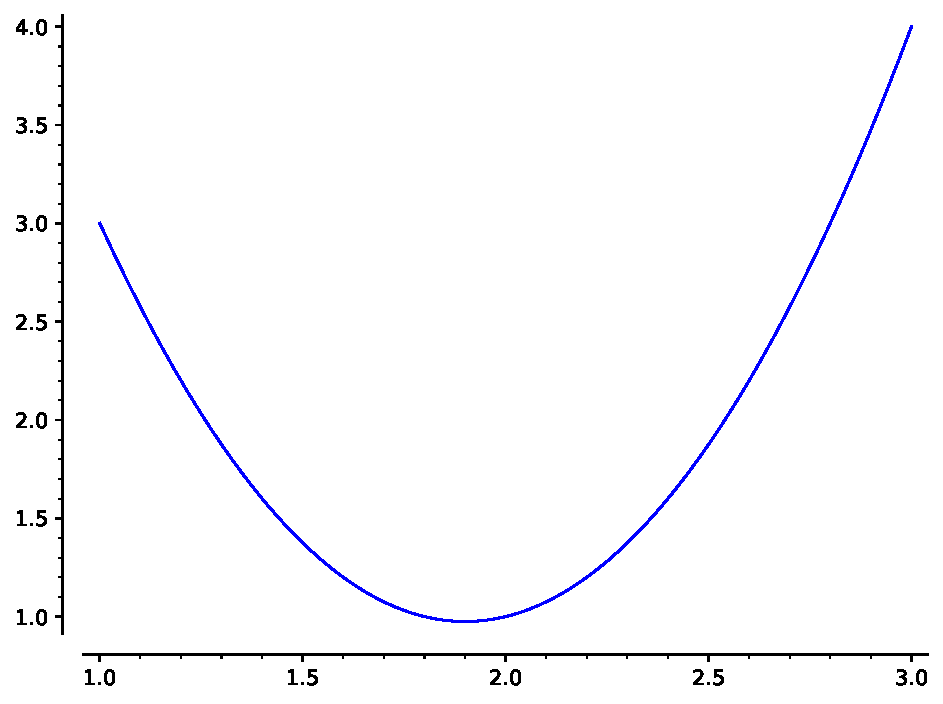
\includegraphics[height=30mm]{pics/plot_lagpol.pdf}
	\begin{block}{Beispiel (fortgesetzt)}
		\begin{itemize}
			\item Wir rechnen direkt nach, da\ss
				\begin{align*}
					L(1)&=3&L(2)&=1&L(3)&=4.
				\end{align*}
			\item Das Polynom hat Grad 2.
		\end{itemize}
	\end{block}
\end{frame}

\begin{frame}\frametitle{\mytitle}
	\begin{block}{Newtonpolynome}
		\begin{itemize}
			\item Seien wiederum $(x_0,y_0),\ldots,(x_n,y_n)$ gegeben.
			\item Die \emph{Newtonbasispolynome} sind definiert durch
				\begin{align*}
					\cN_0(x)&=1\\
					\cN_j(x)&=\prod_{i=0}^{j-1}(x-x_j)&&(j\geq1)
				\end{align*}
			\item Ferner definieren wir rekursiv die \emph{dividierten Differenzen}
				\begin{align*}
					[y_i]&=y_i\\
					[y_i,\ldots,y_{i+j}]&=\frac{[y_{i+1},\ldots,y_{i+j}]-[y_i,\ldots,y_{i+j-1}]}{x_{i+j}-x_i}
				\end{align*}
				mit der Konvention $\frac{0}{0}=0$.
		\end{itemize}
	\end{block}
\end{frame}

\begin{frame}\frametitle{\mytitle}
	\begin{block}{Newtonpolynome (fortgesetzt)}
		\begin{itemize}
			\item Das \emph{Newtonpolynom} ist nun definiert durch
				\begin{align*}
					N(x)&=\sum_{j=0}^n[y_0,\ldots,y_j]\cN_j(x).
				\end{align*}
			\item Der Grad des Polynoms ist $\leq n$.
		\end{itemize}
	\end{block}
\end{frame}

\begin{frame}\frametitle{\mytitle}
	\begin{block}{Beispiel}
		\begin{itemize}
			\item Gegeben seien wieder die Punkte $(1,3)$, $(2,1)$, $(3,4)$.
			\item Wir berechnen
				\begin{align*}
					\cN_0(x)&=1&
					\cN_1(x)&=x-1&
					\cN_2(x)&=(x-1)(x-2)=x^2-3x+2
				\end{align*}
			\item Ferner $[y_0]=3$ sowie
				\begin{align*}
					[y_0,y_1]&=\frac{[y_1]-[y_0]}{x_1-x_0}=\frac{1-3}{2-1}=-2\\
					[y_1,y_2]&=\frac{[y_2]-[y_1]}{x_2-x_1}=\frac{4-1}{3-2}=3\\
					[y_0,y_1,y_2]&=\frac{[y_1,y_2]-[y_0,y_1]}{x_2-x_0}=\frac{3-(-2)}{3-1}=\frac{5}{2}
				\end{align*}
			\item Einsetzen ergibt $N(x)=\frac{5}{2}x^2-\frac{19}{2}x+10$.
		\end{itemize}
	\end{block}
\end{frame}

\begin{frame}\frametitle{\mytitle}
	\begin{block}{Bernsteinpolynome}
		\begin{itemize}
			\item Das \emph{$i$-te Bernsteinpolynom vom Grad $n$ auf $[0,1]$} ist 
				\begin{align*}
					B_{i}(x)&=\binom ni x^i(1-x)^{n-i}.
				\end{align*}
			\item Das \emph{$i$-te Bernsteinpolynom vom Grad $n$ auf $[a,b]$} ist 
				\begin{align*}
					B_i(x;a,b)&=B_i\bcfr{x-a}{b-a}.
				\end{align*}
		\end{itemize}
	\end{block}
\end{frame}

\begin{frame}\frametitle{\mytitle}
	\begin{block}{Proposition}
			Zu jedem Polynom $f(x)=\sum_{i=0}^na_ix^i$ gibt es $b_0,\ldots,b_n\in\RR$, so da\ss
			\begin{align*}
				f(x)=\sum_{i=0}^nb_iB_i(x).
			\end{align*}
	\end{block}
\end{frame}

\begin{frame}\frametitle{\mytitle}
	\begin{block}{Satz}
		Sei $f:[0,1]\to\RR$ eine stetige Funktion.
		Dann gilt
		\begin{align*}
			\lim_{n\to\infty}\sup_{x\in[0,1]}\abs{f(x)-\sum_{i=0}^nf(i/n)B_i(x)}=0.
		\end{align*}
	\end{block}
\end{frame}

\begin{frame}\frametitle{\mytitle}
	\begin{block}{Zusammenfassung}
		\begin{itemize}
			\item Wir haben drei verschiedene Ans\ae tze zur Polynominterpolation kennengelernt:
				\begin{itemize}
					\item Lagrangepolynome,
					\item Newtonpolynome,
					\item Bernsteinpolynome.
				\end{itemize}
			\item Mit Hilfe der Bernsteinpolynome k\oe nnen beliebige stetige Funktionen auf $[0,1]$ angen\ae hert werden.
		\end{itemize}
	\end{block}
\end{frame}

\end{document}
